\paragraph{QuizziPedia::Front-End::Services::LangService}
\begin{figure}[ht]
	\centering
	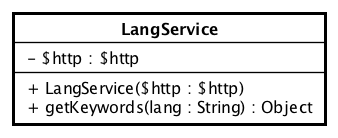
\includegraphics[scale=0.60]{UML/Classi/Front-End/QuizziPedia_Front-end_Services_LangService.png}
	\caption{QuizziPedia::Front-End::Services::LangService}
\end{figure}\FloatBarrier
\begin{itemize}
	\item \textbf{Descrizione}: questa classe permette di gestire la lingua nella quale si è scelto di utilizzare l'applicazione;
	\item \textbf{Utilizzo}: fornisce delle funzionalità per recuperare la giusta traduzione delle pagine;
	\item \textbf{Relazione con altre classi:}
	\begin{itemize}
		\item \textit{IN} \texttt{AppRun}: classe che permette l'avvio dell'applicazione.
	\end{itemize}
	\item \textbf{Attributi:}
	\begin{itemize}
		\item \texttt{-} \texttt{\$http: \$http} \\ Campo dati che contiene un riferimento al servizio \$http che permette la comunicazione con il protocollo \textit{HTTP\ped{G}}.
	\end{itemize}
	\item \textbf{Metodi:}
	\begin{itemize}
		\item \texttt{+} \texttt{LangService(\$http: \$http)} \\ Metodo costruttore della classe. \\
		\textbf{Parametri}:
		\begin{itemize}
			\item \texttt{\$http: \$http} \\ Campo dati contenente un riferimento al servizio \$http creato da \textit{AngularJS\ped{G}} per facilitare la comunicazione mediante protocollo \textit{HTTP\ped{G}}.
		\end{itemize}
		\item \texttt{+} \texttt{getKeywords(lang: String): Object} \\Metodo che ritorna la lista di tutte le keywords nella lingua richiesta.\\
		\textbf{Parametri}:
		\begin{itemize}
			\item \texttt{lang: String} \\ Parametro che indica la lingua delle \textit{keywords\ped{G}} da restituire.
		\end{itemize}
	\end{itemize}
\end{itemize}